\subsection{График результата}

Ниже изображён график полученной формулы линейной регрессии:
\[
    f(x)=4.948 - 3.935x + 0.985x^2
\]

Для сравнения результата с выборкой на график нанесены точки вида \( (X,Z) \), которые соответствуют данным из исходной выборки.

\begin{figure}[H]
\centering
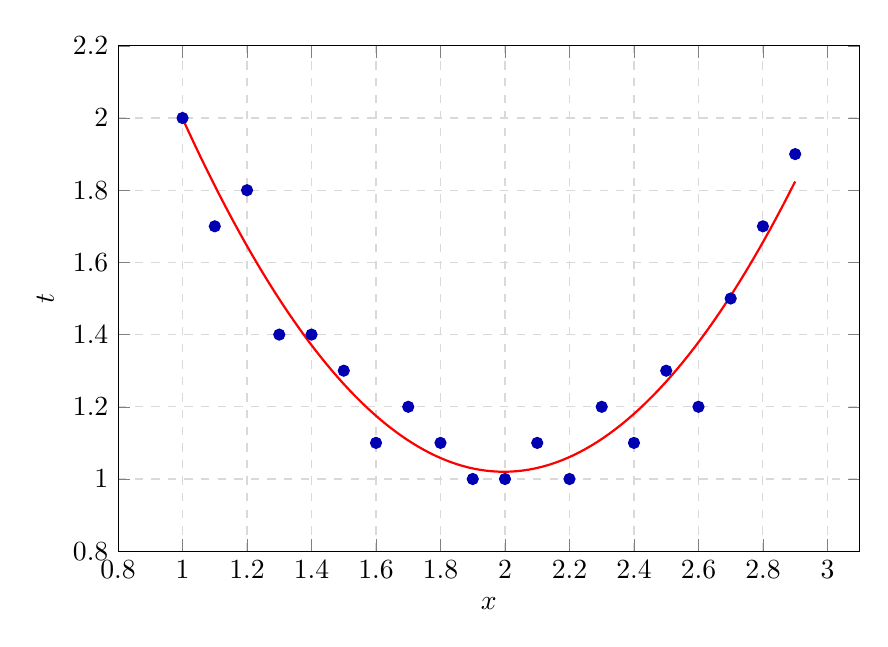
\begin{tikzpicture}
\begin{axis}[
    xlabel={$x$},
    ylabel={$t$},
    grid=both,
    grid style={dashed, gray!30},
    legend pos=north west,
    width=11cm, height=8cm,
    xmin=0.8, xmax=3.1,
    ymin=0.8, ymax=2.2,
]

% 1. Plot the sample points (dots)
\addplot[
    only marks,
    mark=*,
    mark size=2pt,
    blue!70!black
] coordinates {(1.0,2.0) (1.1,1.7) (1.2,1.8) (1.3,1.4) (1.4,1.4) (1.5,1.3) (1.6,1.1) (1.7,1.2) (1.8,1.1) (1.9,1.0) (2.0,1.0) (2.1,1.1) (2.2,1.0) (2.3,1.2) (2.4,1.1) (2.5,1.3) (2.6,1.2) (2.7,1.5) (2.8,1.7) (2.9,1.9)};

% 2. Plot the regression function mathematical expression
\addplot[
    red,
    thick,
    domain=1.0:2.9,
    samples=100
] {4.9483 + (-3.9349*x) + (0.9854*x^2)};

\end{axis}
\end{tikzpicture}
\caption{Результат линейной регрессии методом наименьших квадратов}
\end{figure}